\section{The \grackle{} Chemistry and Cooling Library}

\begin{figure}[h]
\begin{center}
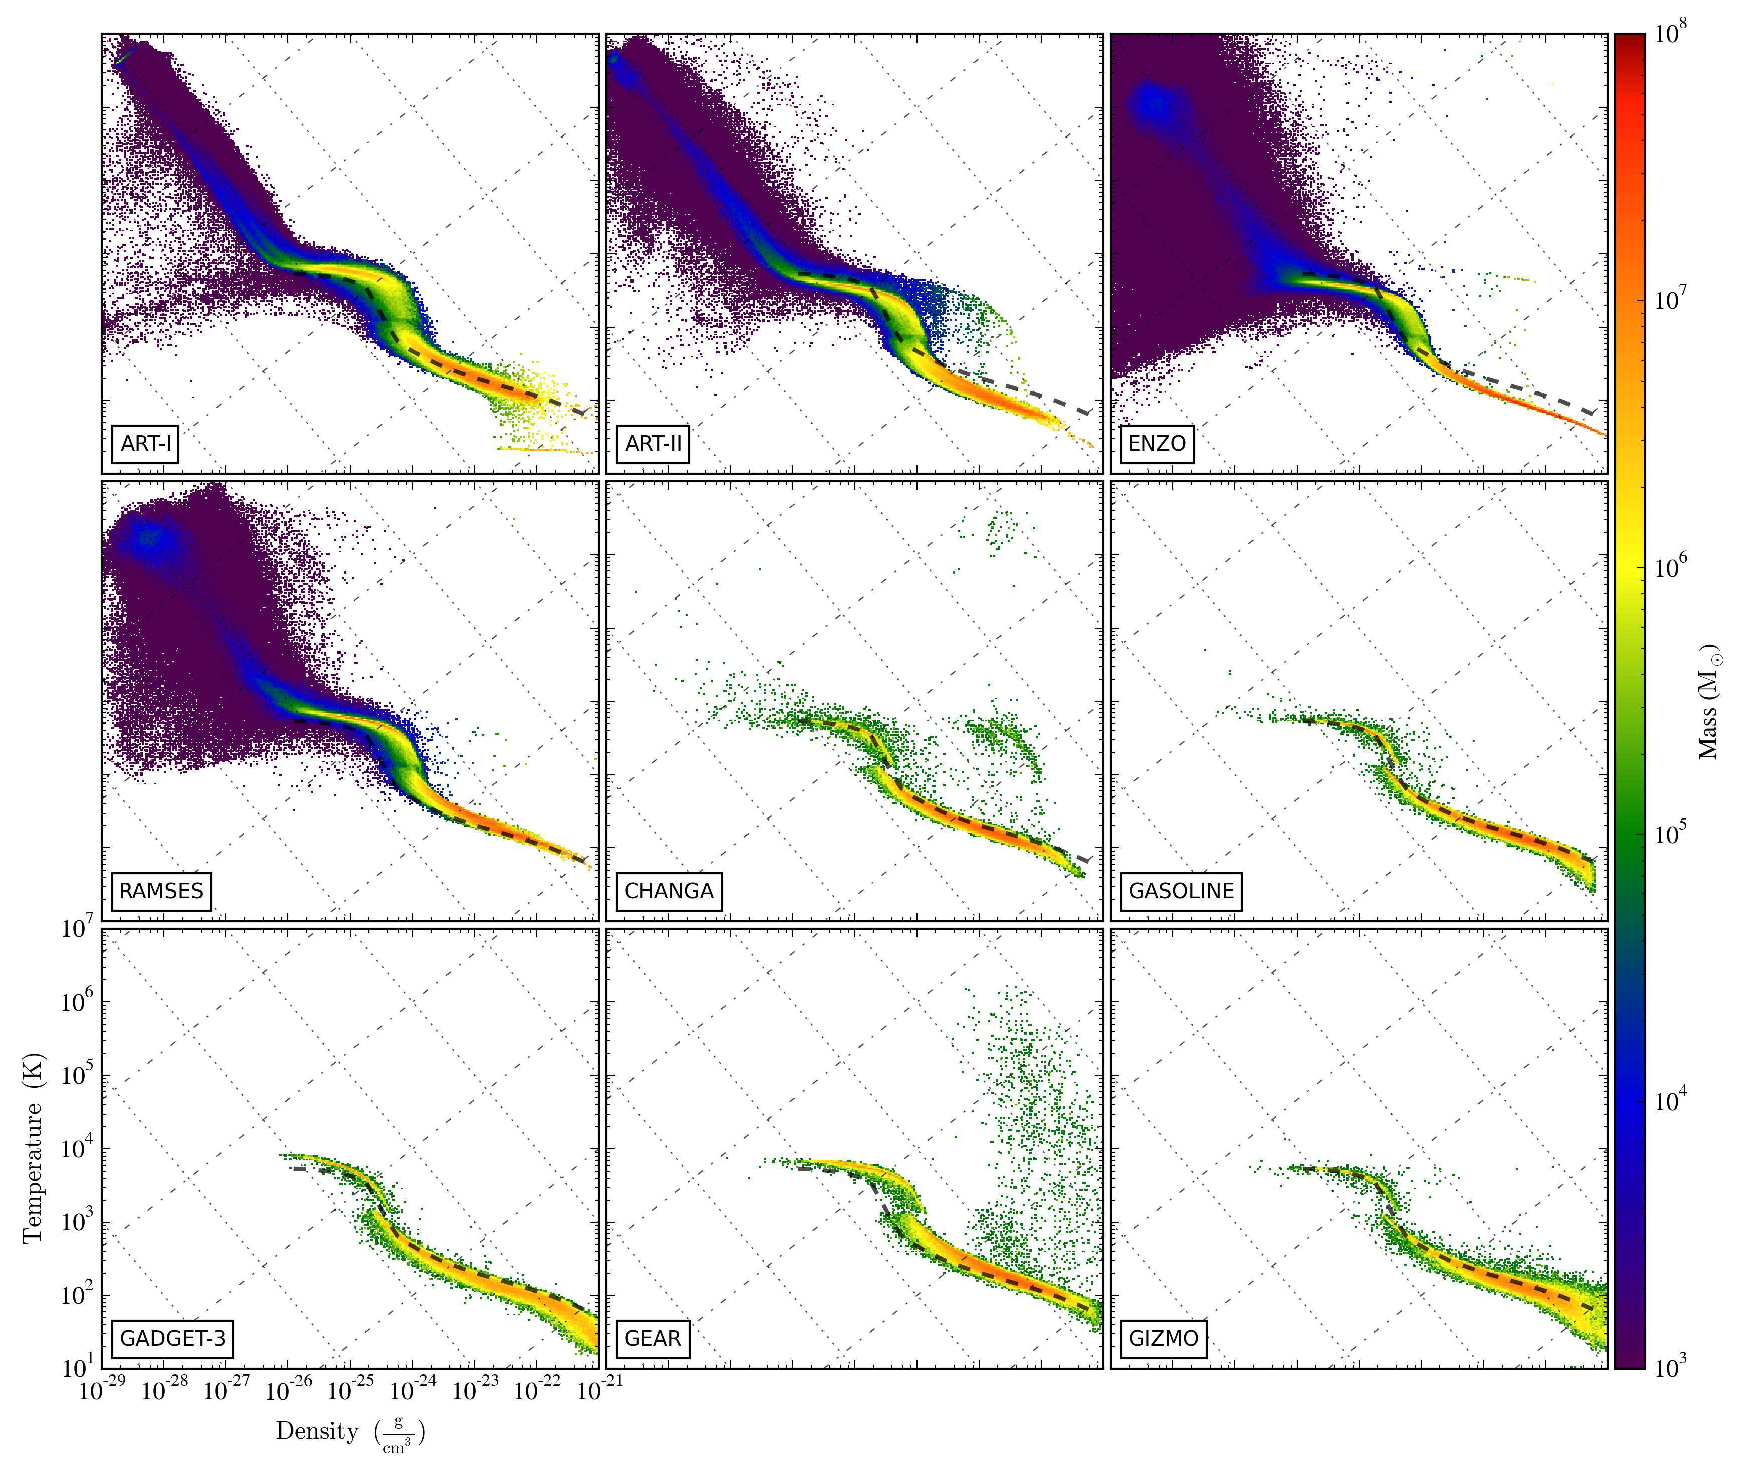
\includegraphics[width=0.92\textwidth]{figures/fig17.eps}
\caption{Figure 17 from \citet{2016ApJ...833..202K}, showing a
  comparison of nine simulation codes in the AGORA project, all using
  \grackle{}.  The panels show the probability distribution function
  in bins of density and temperature for the gas in isolated galaxy
  simulations.  Each simulation used an identical idealized setup,
  prescriptions for star formation and feedback, and radiative cooling
  provided by the \grackle{} library.}
\label{fig:AGORA}
\end{center}
\vspace*{-2\baselineskip}
\end{figure}

The \grackle{} project
\citep[][\url{https://grackle.readthedocs.io}]{2017MNRAS.466.2217S} is
an open-source library for computing the chemistry and radiative
cooling in astrophysical simulations and models.  The
\grackle{} library exposes functions necessary for computing the
thermal and chemical evolution of a collection of fluid elements carried by a
simulation.  These fluid elements can be either Eulerian (cells),
Lagrangian (particles), or a hybrid (e.g., moving mesh) with
application programming interfaces (APIs)
existing for codes written in C, C++, Fortran, and Python.  The
physical processes covered by the solver make it applicable to a broad
range of astrophysical topics, including star and galaxy formation, the
evolution of the intergalactic medium, and galaxy clusters.  Among
other metrics, the utility of \grackle{} can be demonstrated in two
important ways.  First, \grackle{} is a key component of the AGORA
\citep{2014ApJS..210...14K, 2016ApJ...833..202K} simulation comparison
project.  Comparing nine different simulation codes over multiple
galaxy formation problems, the AGORA project is the first
undertaking to include such a large fraction of the galaxy formation research
community.  An example of this cross-platform comparison enabled by
\grackle{} is shown in Figure \ref{fig:AGORA}.  Second, \grackle{} has
seen widespread adoption and use outside of participation in AGORA.
In total, \grackle{} has been adopted by at least 14 different
simulation codes:
AREPO, ART-I, ART-II, CHANGA, Cosmos++, Enzo, Gadget, GAMER, GASOLINE, Gear,
Gizmo, RAMSES, SPHS, and SWIFT
\citep{2010MNRAS.401..791S, 1999PhDT........25K, 2002ApJ...571..563K,
2008ApJ...672...19R, 2004NewA....9..137W, 2006MNRAS.373.1074S,
2003ApJS..147..177A, 2005ApJ...635..723A, 2014ApJS..211...19B,
2005MNRAS.364.1105S, 2010ApJS..186..457S, 2004NewA....9..137W,
2012A&A...538A..82R, 2012ASPC..453..141R, 2015MNRAS.450...53H,
2002A&A...385..337T, 2012MNRAS.422.3037R, 2013arXiv1309.3783G,
2016arXiv160602738S}.

\noindent
{\bf As an open-source project, \grackle{} plays two major roles:}
\begin{enumerate}
\item It provides access via a universal API to necessary functionality
that can be difficult for individual research groups to develop or
maintain on their own.  This increases overall productivity and
enables comparison and collaboration.
\item By actively encouraging contribution though personal engagement
and open-source software best practices, the widely adopted API serves
as a conduit for dissemination of new methods and research results to
the community.
\end{enumerate}
However, for \grackle{} to continue to be a useful resource, key
development projects must be undertaken to ensure that the code is
more inviting to new contributors, does not become a bottleneck
for effective utilization of next-generation computing facilities, 
and is flexible enough to be adapted to new areas of research.
The purpose of this CSSI Software Elements proposal is to support a
series of specific infrastructure and feature development tasks
necessary to keep up with the demands of current users, broaden
applicability to new domains and user bases, and to make \grackle{} a
self-sustaining community project by the end of the 
three-year grant period.  The proposed tasks and their order of
completion have been designed to yield regular major code releases at
the end of each year.
%% The proposed tasks and their order of
%% completion have been designed to incrementally make the code more
%% attractive to external contribution and adoption by a wider audience.
%% The completion of each task will be marked by a major release of the
%% code.

\subsection{\grackle{} API}\label{sec:arch}

\grackle{} is a full-featured solver for gas chemistry and radiative
cooling with an API that is designed to minimize backward
compatibility issues and is straightforward to implement in simulation
codes written in C, C++, Fortran, and Python.  All functionality is
parallelized with OpenMP and can be used in hybrid MPI/OpenMP
frameworks.  To aid in semi-analytical
modeling and debugging of new features, it also includes a Python
interface with additional functionality.  Below, we detail the
features included and the functions provided to the user.

\grackle{} provides a non-equilibrium primordial chemistry solver for
atomic and molecular species of H, D, and He, including H$_{2}$
formation via three-body reactions \citep{2002Sci...295...93A,
2011ApJ...726...55T} and on dust-grain surfaces
\citep{1979ApJS...41..555H, 2000ApJ...534..809O, 2014ApJ...783...75M},
H$_{2}$ formation 
heating \citep{2009Sci...325..601T}, collision-induced H$_{2}$
emission \citep{2004MNRAS.348.1019R}, and HI
\citep{2013MNRAS.430.2427R} and H$_{2}$ \citep{2012MNRAS.425L..51W}
self-shielding.  The cooling from heavy elements up to atomic number
30 (Zn) is calculated by interpolating over tables of cooling and
heating rates created with the photo-ionization software,
\texttt{Cloudy} \citep{2013RMxAA..49..137F}.  These
tables are stored in HDF5 files included with the source.  For
increased speed at the expense of accuracy, the cooling from
primordial elements can also be computed using these tables.  In
addition to tables calculated assuming collisional ionization only
(i.e., no incident radiation), cooling tables have been created for two
different UV background models, those of \citet{2009ApJ...703.1416F}
and \citet{2012ApJ...746..125H}, in order to mimic the effects of
reionization.  For radiative transfer codes or simulation codes that
support radiation hydrodynamics, \grackle{} also allows the user to supply
photo-ionization and photo-heating rates for each computational
element.  Finally, arrays of arbitrary specific and volumetric heating
rates may be supplied to account for heating from stellar feedback
models and additional radiation sources.

The \grackle{} library exposes five primary functions useful to a
hydrodynamic simulation: 1) \texttt{solve\_chemistry} for iterating
the chemistry network and updating the species densities and internal
energy over a given time-step, and 2)
\texttt{calculate\_cooling\_time}, 3) \texttt{calculate\_pressure}, 4)
\texttt{calculate\_temperature}, and 5) \texttt{calculate\_gamma} for
computing the instantaneous cooling time, thermal pressure,
temperature, and ratio of specific heats, respectively.  Most of the
code's behavior is controlled by run-time parameters stored within a C
\texttt{struct} that is accessible from the main \grackle{} header
file.  The solver can be run with varying levels of sophistication,
including fully tabulated cooling, atomic chemistry only (6-species,
H, H$^{+}$, He, He$^{+}$, He$^{++}$, e$^{-}$), and additional tiers of
molecular chemistry (9-species adding H$_{2}$, H$_{2}^{+}$, H$^{-}$
and 12-species adding D, D$^{+}$, and HD).  Each of these, and other
optional features, requires a different number of fields to be carried
by the simulation code.  This functionality is exposed through
an API that has been designed to minimize the possibility of future
development breaking backward compatibility.

%% To maintain a single function signature,
%% regardless of chosen settings, field arrays are attached to pointers
%% within a C \texttt{struct} that is passed to the primary functions.
%% With this technique, new features requiring additional fields can be
%% added without altering function signatures, making the code
%% effectively backward compatible indefinitely.  This was an explicit
%% design decision made by the project to minimize future work required
%% by simulation codes using \grackle{}.

%\begin{wrapfigure}[20]{l}{0.50\textwidth}
%\vspace*{-2\baselineskip}
\begin{figure}
\begin{center}
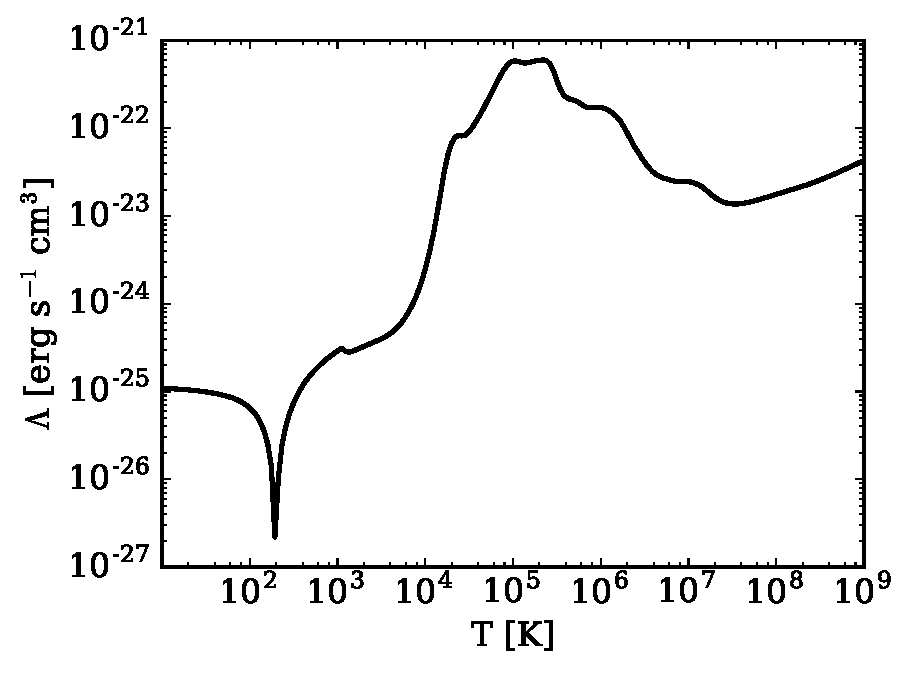
\includegraphics[width=0.48\textwidth]{figures/cooling_rate.pdf}
\caption{The cooling rate vs. temperature calculated by \grackle{}
  (using the \texttt{cooling\_rate.py} example script) for
  a gas with density of 10$^{-24}$ g/cm$^{-3}$ and solar metallicity,
  exposed to a radiation field described by the \citet{2012ApJ...746..125H} UV
  background model at redshift, z = 0.}
\label{fig:cooling-rate}
\end{center}
\vspace*{-1\baselineskip}
\end{figure}
%\end{wrapfigure}

\begin{figure}
\centering
\begin{subfigure}{.48\textwidth}
  \centering
  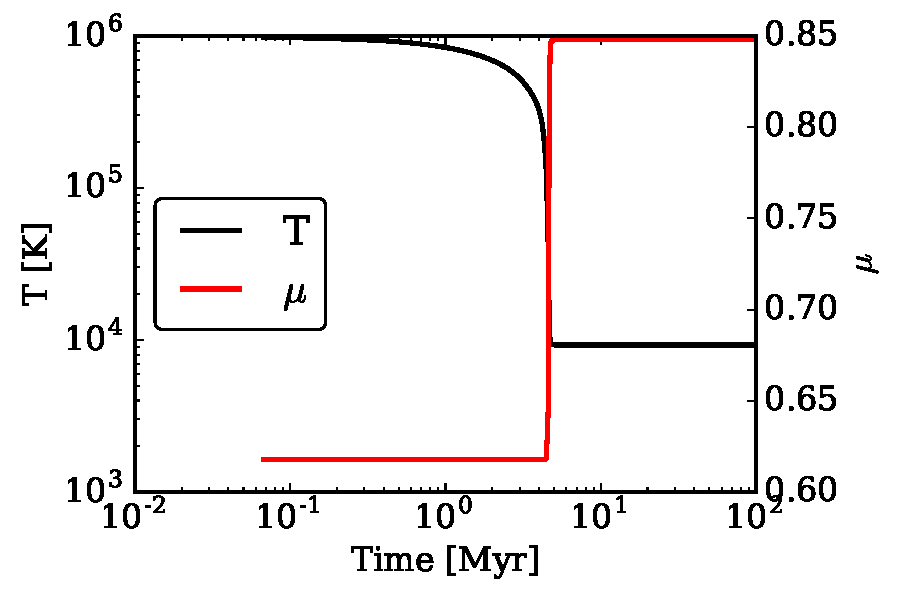
\includegraphics[width=0.98\textwidth]{figures/cooling_cell.pdf}
  \caption{Constant density model (\texttt{cooling\_cell.py}).}
  \label{fig:cooling-cell}
\end{subfigure}%
\begin{subfigure}{.48\textwidth}
  \centering
  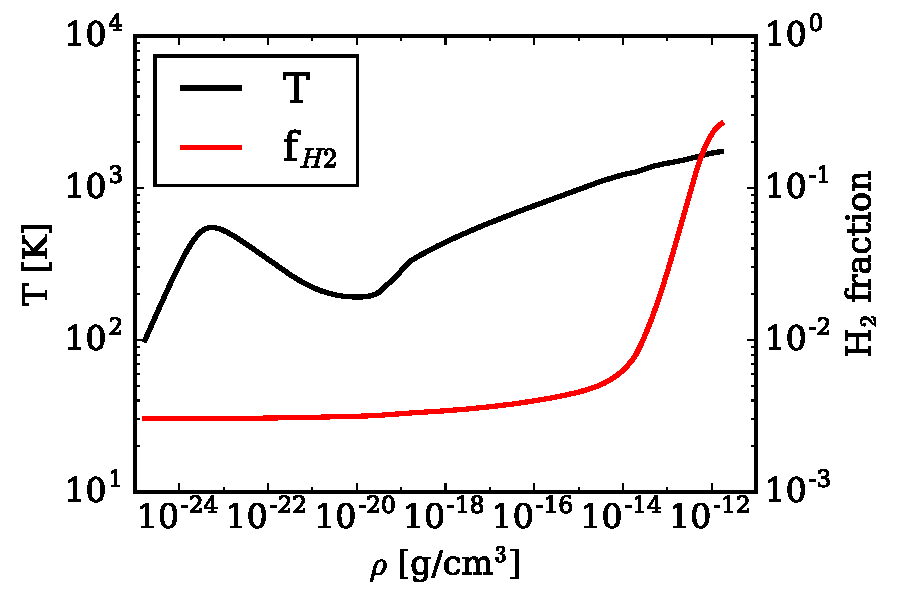
\includegraphics[width=0.98\textwidth]{figures/freefall.pdf}
  \caption{Free-fall collapse model (\texttt{freefall.py}).}
  \label{fig:freefall}
\end{subfigure}%
\caption{Example output from Python scripts included in the \grackle{}
  source using \texttt{pygrackle}'s helper functions for evolving
  fluid containers.}
\label{fig:evolve}
\vspace*{-1\baselineskip}
\end{figure}

\grackle{} has been designed to maximize scientific productivity on
high performance computing systems while maintaining an interface that
is immediately useful to people at many different levels of
experience.
All of the above functionality is easily accessible to codes written
in C, C++, and Fortran.  The \grackle{} source comes with compilable,
runnable examples in each of the above languages demonstrating all
available functions.  In addition, a Python module, \texttt{pygrackle},
is provided, exposing the main functionality as well as additional helper
functions useful in semi-analytic models, such as computing the
thermal evolution of a parcel of gas at constant density or undergoing
free-fall collapse.  Sample Python scripts are included in the source,
the running of which results in a figure of merit (shown in Figures
\ref{fig:cooling-rate} and \ref{fig:evolve}).

\subsection{\grackle{} Architecture}

\grackle{} is built upon widely used packages in the ecosystem of
scientific software.  As a library, the aim is to provide
functionality to the most commonly used programming languages in
scientific computing, namely, C, C++, Fortran, and Python.  The core
library is written in a combination of C and Fortran with the strategy
of using Fortran for the computationally expensive internal machinery
and C for user-facing functions and data storage.  The single
additional dependency is
HDF5\footnote{\url{https://www.hdfgroup.org/HDF5/}}, used for reading
cooling, heating,
and UV background rate data from input files.  HDF5 was chosen because
\grackle{}'s input files contain many data tables and the hierarchical
format makes them easily discoverable without prior knowledge of the
layout, allowing them to be easily reused by other codes.  The Python
interface makes use of a number of widely used Python packages, including
\texttt{NumPy}, \texttt{Cython}, and
\yt{}\footnote{\url{http://www.numpy.org/}, \url{http://cython.org/},
  and \url{http://yt-project.org/}, respectively} \citep[][an SI2-funded
project]{2011ApJS..192....9T}.  In
addition, the project infrastructure relies on the following packages:
Mercurial as the version control system; BitBucket.org to host the
main repository; Sphinx for building documentation; readthedocs.org to
host the latest build of the documentation; pytest for testing; and BitBucket
Pipelines for continuous integration testing.

\subsubsection{The Core Library}
\label{sec:core-library}

\noindent
{\bf Methodology}
Chemistry networks are challenging to solve because the time-scales of
reactions involved vary by many orders of magnitude.  These ``stiff''
networks are often solved using implicit methods, as they are able to
take longer time-steps than explicit methods, which are limited by the
shortest time-scale within the network.  However, a number of factors
can make an explicit scheme more attractive in certain situations,
particularly when the network is a component in a more complex physical
model governed by additional time-scales, as is the case here
\citep{2012JCoPh.231.5266G}.  Such factors include a higher
computational cost per solve with an implicit solver, steeper scaling
with the number of species, and the potential for hand-tuning of
explicit solvers for greater speed.  \grackle{} solves the primordial
chemistry network using an explicit method with a series of
optimizations shown by \citet{1997NewA....2..181A} to achieve
significant speedup with minimal cost to stability.  These
optimizations include replacing the fastest evolving species with
their thermal equilibrium values, tuning the order in which species
are updated, and switching between analytical and numerical time
derivatives when the system is close to equilibrium.  The time-steps
passed to \grackle{} from the simulation code are often much longer
than the relevant internal
time-scales.  To account for this, \grackle{} iterates in
``subcycles'' over time-steps limited by no more than 10\% of the
cooling time ($e/\dot{e}$) and chemical time-scales ($n/\dot{n}$) for
neutral H and for electrons.

\begin{figure}[h]
\centering
\begin{subfigure}{.54\textwidth}
  \centering
  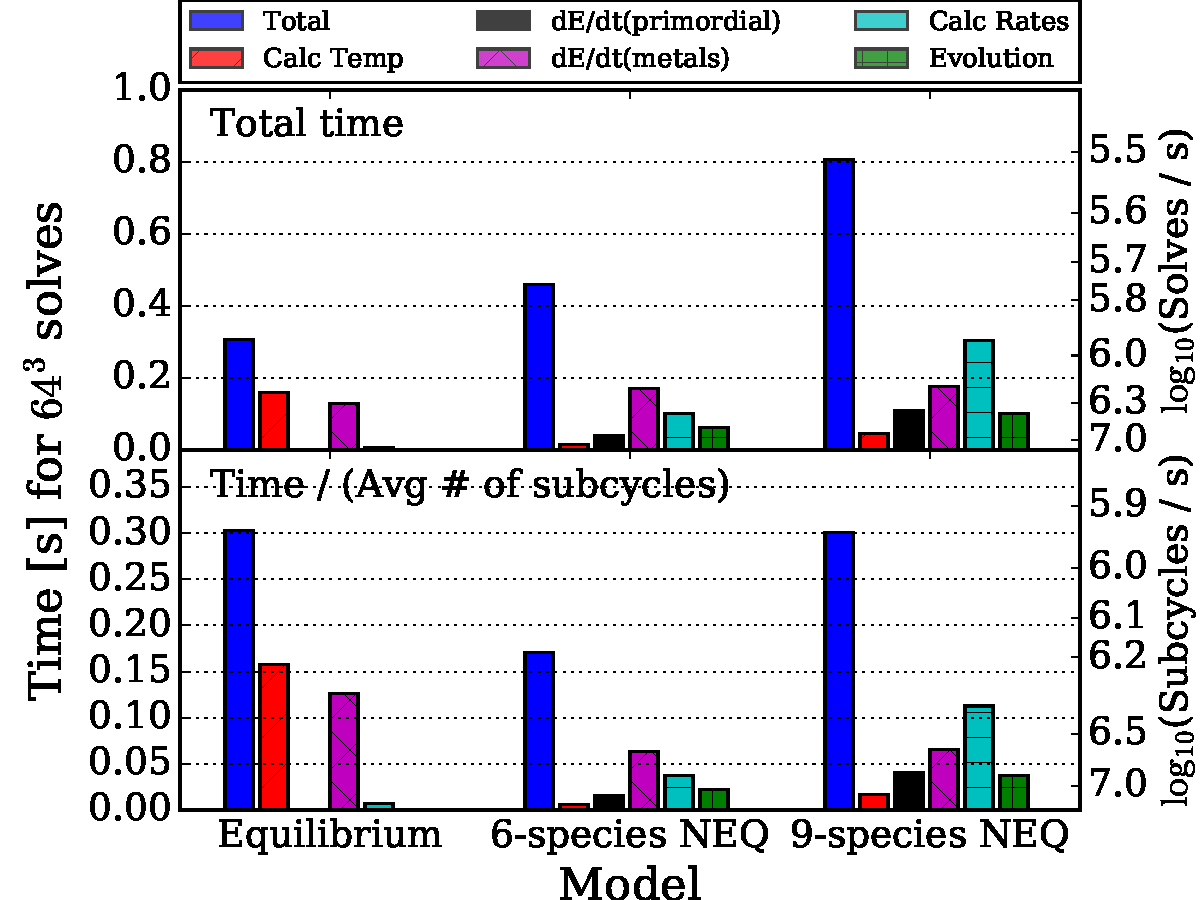
\includegraphics[width=0.98\textwidth]{figures/performance.pdf}
  \caption{Serial performance - Top: time
    to integrate a fluid container with 64$^{3}$ elements, with the
    tabulated cooling (``equilibrium'', left), the atomic chemistry
    (``6-species'', middle), and H$_{2}$ molecular chemistry
    (``9-species'', right) models.  Bottom: time normalized by the
    average subcycles per cell.  Colors denote the full solve
    (blue), temperature calculation (red), primordial (black) and metal
    (magenta) cooling rate calculation, and interpolation of chemistry
    rate coefficients (cyan).}
  \label{fig:single-proc}
\end{subfigure}%
\hspace{0.02\textwidth}
\begin{subfigure}{.42\textwidth}
  \centering
  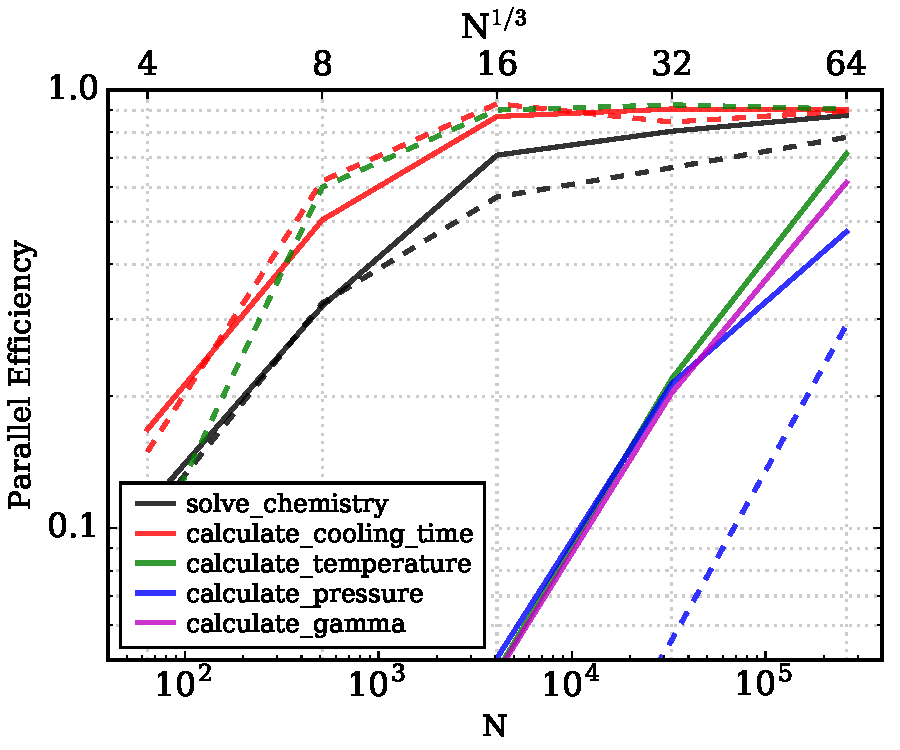
\includegraphics[width=0.98\textwidth]{figures/openmp.pdf}
  \caption{OpenMP parallel efficiency vs. size of fluid container for
    20 threads.  Solid lines show the molecular
    chemistry solver and dashed lines show the tabulated, equilibrium
    model.  For all expensive routines, the efficiency reaches
    $\sim$60\% to 90\% for $16^3$ cells and $\sim$80\% to 90\% for
    $64^3$ cells.}
  \label{fig:openmp}
\end{subfigure}%
\caption{Figures 5 (left) and 6 (right) from
  \citet{2017MNRAS.466.2217S}, showing the single processor
  performance and OpenMP efficiency of \grackle{}'s solvers.}
\label{fig:performance}
\vspace*{-1\baselineskip}
\end{figure}

In addition to the primordial chemistry and cooling, the contribution
to the total cooling rate by metals is calculated by linearly
interpolating over pre-computed tables of heating and cooling rates,
following the method of \citet{2008MNRAS.385.1443S}.
The metal cooling component is calculated within the same subcycle
iteration as the chemistry solver and contributes to the cooling time
time-step limiter.
If using a UV background model, (e.g.,
\citet{2009ApJ...703.1416F} or \citet{2012ApJ...746..125H}),
additional tables also provide photo-ionization, photo-dissociation,
and photo-heating rates for the various atomic and molecular species
in the primordial chemistry as a function of redshift.
The tables distributed with the source code are calculated with the
photo-ionization code, \texttt{Cloudy}, but can in principle be
generated by other similar codes, such as \texttt{Mappings III}
\citep{1993ApJS...88..253S}.

\noindent
{\bf Implementation}
All user-facing \grackle{} functions are written in C due
to the relative simplicity of calling C routines from other
languages, particularly C++ and Fortran.  Most of \grackle{}'s
internal functionality is written in Fortran to make use of the
language's efficient loop and array operations.
The internal machinery is optimized to work with a set of arrays of
densities and internal energies, referred to collectively as a ``fluid
container'', where the arrays can represent either a three-dimensional
grid with inactive ghost zones or a one-dimension set of particles.
The solvers are designed to make the best possible use of cache by
operating on field data in the order in which it is stored in memory.
The core chemistry and cooling computations are performed on
contiguous sub-segments of the field arrays to allow for loops to be
unrolled by compilers for more efficient vector operations.  For
three-dimensional grids, these sub-segments are pencil-beams of all $i$
values for given values $k$ and $j$ in an $i\times j\times k$ cube.
For 1D arrays of particles, analogous divisions can be used to break
the arrays into multiple sub-segments to be passed to the core
functions.

\noindent
{\bf Performance}
In Figure \ref{fig:single-proc}, we
display performance results for \grackle{}'s different solvers.  For
this test, we initialize a 3D fluid container with 64$^{3}$ elements
with density, temperature, and metallicity varying smoothly in each
dimension over the following ranges: $\log (n_{\rm H} /
\textrm{cm}^{-3}) = [-1, 3]$, $\log (T/\textrm{K}) = [1, 8]$, and
$\log (Z/Z_\odot) = [-4, 0]$.  We then evolve the fluid container for
500 years (through repeated called to \texttt{solve\_chemistry}) on a
single core of an Intel Xeon ``Westmere'' E5645 CPU (dual-processor with
6 cores/processor at 2.4 GHz).  On this machine, \grackle{} performs
roughly 0.5-1$\times10^{6}$ full solves per second and at least
10$^{6}$ subcycles per second, depending only slightly on the choice
of solver.  Due to a lack of similar packages, an absolute evaluation
of this performance is difficult.  However, a comparison can be made
to the performance of the \texttt{Enzo} simulation code as a whole.
\citet{2014ApJS..211...19B} perform a weak scaling test of
\texttt{Enzo} on XSEDE's NICS Kraken (a Cray XT4 with quad-core AMD
Opteron CPUs at 2.3 GHz) with a simulation including gravity,
hydrodynamics, and a chemistry solver analogous to \grackle{}'s atomic
solver.  They find that \texttt{Enzo} optimally reaches about 10$^{5}$
full cell updates per second, suggesting that \grackle{} would consume
approximately 20-25\% of the computational cost.

\noindent
{\bf Parallelism}
Because \grackle{}'s functionality requires no communication and is
fully thread-safe once initialized, the library can be easily used
within a simulation code parallelized with a message passing framework
like MPI.  Additionally, all of \grackle{}'s functions are
parallelized with OpenMP by threading the outer loops over which the
solvers are called to operate on the field array sub-segments.  This
allows the library to work within hybrid MPI/OpenMP frameworks, such
as that adopted by the latest version of \texttt{Gadget}.
In Figure \ref{fig:openmp}, we show the OpenMP efficiency of
\grackle{}'s functions for the most and least complex versions
of the solver.  Here, we define parallel efficiency as the ratio of
multi- to single-thread performance.  The test is run using 20 OpenMP
threads on an Intel Xeon E5-2670 v2 CPU (dual-processor with 10
cores/processor at 2.50 GHz) for fluid container sizes from 4$^{3}$ to
64$^{3}$.  For only 16$^{3}$ fluid elements, the efficiency is 60-90\%
for all computationally expensive routines.  The four routines that
show relatively poor efficiency are very inexpensive (for example, see
the 9-species, molecular version of \texttt{calculate\_temperature} as
shown in Figure \ref{fig:single-proc}) and so contribute negligibly to
the total cost.  This parallelism can also be beneficial to pure-MPI codes
where memory requirements force the use of fewer than the total number
of cores on a node, as is often the case.

\subsubsection{\texttt{pygrackle}: The Python Interface}

The Python interface, \texttt{pygrackle}, provides a lower barrier to
entry for accessing \grackle{}'s functionality and thus can be
useful for semi-analytical models \citep[e.g.,][]{2016ApJ...820...71C,
2016MNRAS.459.4209A}, debugging, and education.  The
\texttt{pygrackle} package is distributed with the \grackle{} source
and can be installed once the library has been compiled.  The
additional Python packages on which \texttt{pygrackle} is built
(\texttt{NumPy}, \texttt{Cython}, and \yt{}) are
installable by popular Python package managers, like \texttt{Conda}
and \texttt{pip}.

\texttt{pygrackle} uses an Object-Oriented design centered around
\texttt{FluidContainer} objects.  Analogous to the C \texttt{struct}
by which fields are passed to the \grackle{} library functions, the
\texttt{FluidContainer} object stores field values as \texttt{NumPy}
arrays.  The field arrays use an enhanced version of the
\texttt{NumPy} array, provided by the \yt{} package, that allows
the values to have units that can be expressed and converted
symbolically.  For example, an array, \texttt{x}, of densities in units of
g/cm$^{3}$, can undergo unit conversion by doing:
\texttt{x.to("Msun/kpc**3")}.  The core \grackle{} functions exist as
class methods hanging off the \texttt{FluidContainer} object.  For
example, to calculate the cooling time for a \texttt{FluidContainer}
object, \texttt{fc}, the syntax is
\texttt{fc.calculate\_cooling\_time()}.  The interface layer
connecting the high-level Python data structures to \grackle{}'s C
functions is written in \texttt{Cython}.

\subsection{Community and Usage Metrics}

The first stable version of the \grackle{} library was released in
January 2014.  Since that time, the \grackle{} API has been
implemented in 14 simulation codes and has been used in 23 papers
published in the Astrophysical Journal, Monthly Notices of the Royal
Astronomical Society, and Nature.  The topics of these publications
include galaxy, star, and direct collapse black hole formation; dwarf
and disk galaxies; the high redshift interstellar medium; the
Lyman-alpha forest; history of the Milky Way; reionization; supernova
remnants; metal mixing; and turbulence.  This usage has grown steadily
from year to year, with 1 publication using \grackle{} in 2014, 5 in
2015, 11 in 2016, and 6 within the first two months of 2017.  The
\grackle{} mailing list currently has 68 subscribers, increasing by
roughly 15-20 per year.

Much of \grackle{}'s primordial chemistry solver was first developed
by Peter Anninos and collaborators in the mid-1990s
\citep{1997NewA....2..209A, 1997NewA....2..181A} and incorporated into
the simulation code, \texttt{Enzo} \citep[][licensed under the
  3-clause, revised BSD license]{2014ApJS..211...19B} a few
years later.  As a component of \texttt{Enzo}, the chemistry and
cooling solver was developed through contributions made by many in the
\texttt{Enzo} community, including PI Britton Smith and collaborators
Greg Bryan, Matthew Turk, and Simon Glover.  In response to a call for
a ``common physics package'' to enable a large, multi-simulation
comparison project \citep[AGORA,][]{2014ApJS..210...14K,
  2016ApJ...833..202K}, PI Britton Smith extracted the chemistry and
cooling machinery from \texttt{Enzo} and converted it into a
stand-alone, linkable library that included a number of improvements
and additional features.  The first commit made to the \grackle{}
project was in October 2012.  Since then, the project has progressed
under the same philosophy of feature-driven, community development as
it had as a component of \texttt{Enzo}.  In that time, the code has
received commits from 14 different contributors.

This SSE will establish \grackle{} as a vital software element for the
computational astrophysics community.  It will allow the code to adapt
to the latest technologies that will enable the next generation of
simulations.  It will expand the capabilities of \grackle{} to reach a
larger audience and provide a venue for collaboration and
dissemination of new research.
